\section{Solution Overview and Example}
\label{section:solution}

As discussed previously, the sector analysis technique is part of a larger research effort to 
create design tools for high-confidence distributed control system designs.  As such, each element
and technique in our tool suite performs a particular function within a larger model-driven design 
process.  We will briefly cover the design process to highlight potential uses of the online sector
analysis technique, and illustrate our model-based approach with an example.

\begin{enumerate}
 \item Control designers work from requirements and (if possible) a passive decomposition of the
design to create controllers.
 \item Simulink simulations with included sector analysis blocks provide preliminary evidence that
the design satisfies the requirements.
 \item Software modelers import the Simulink design into the Generic Modeling Environment (GME)
\cite{mic:overview}, creating an instance of a model in the ESMoL language.
 \item In ESMoL software designers specify software component interfaces and functions for the
imported Simulink functions, create hardware platform models, map instances of software control 
components to the platform, and specify dependencies and timing information.
 \item A time-triggered schedule is calculated based on the model structure and timing parameters,
and release times are written back into the model for component instances and timed data messages
\cite{sched:analysis}.
 \item With the schedule in the model, control designers can now synthesize a platform-included Simulink model from the ESMoL model
using the TrueTime toolkit\cite{modeling:truetime}.  The sector analysis technique can be applied
to the platform-specific simulation.
 \item Control designers and software modelers iterate over the previous steps to bring the 
platform-specific simulated design into conformity with the requirements.
 \item Software testers synthesize controller software from the models and deploy it to a 
hardware-in-the-loop simulation for more detailed integration and analysis.  The sector analysis 
technique applies at this stage as well.  The model-based analysis and generation approach makes 
rapid redesign and re-assessment straightforward when needed.
 \item The deployed software and hardware are tested in the actual environment, again using sector
analysis if appropriate. Often the final integration of the controller into the physical environment
makes assessment much more costly, as needed data may be difficult or impossible to get (hence the
focus on simulation).  If our platform-specific and hardware-in-the-loop simulations are sufficiently
detailed, we should be able to avoid major surprises in the final deployment.
\end{enumerate}


\begin{figure}[htb]
\centering
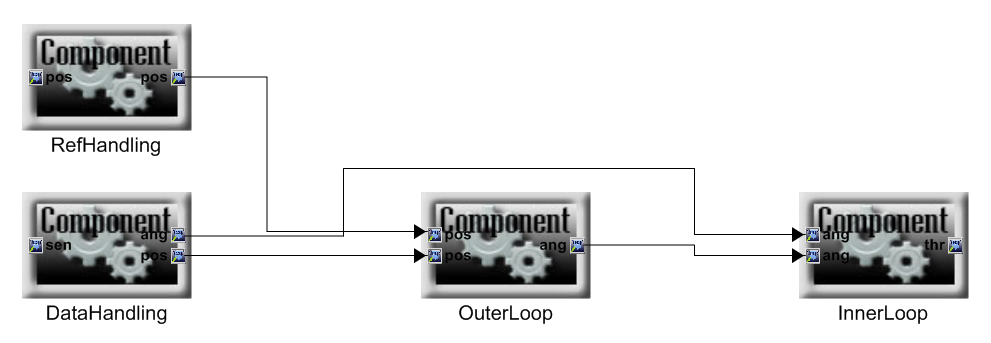
\includegraphics[width=\columnwidth]{figures/quadrotor_log_arch}
    \caption{Deployment: The ESMoL logical architecture model specifies data
dependencies between software component instances. The ports on the blocks
represent data messaging interfaces into and out of the component.}
    \label{fig:qr_log_arch}
\end{figure}

\begin{figure}[htb]
\centering
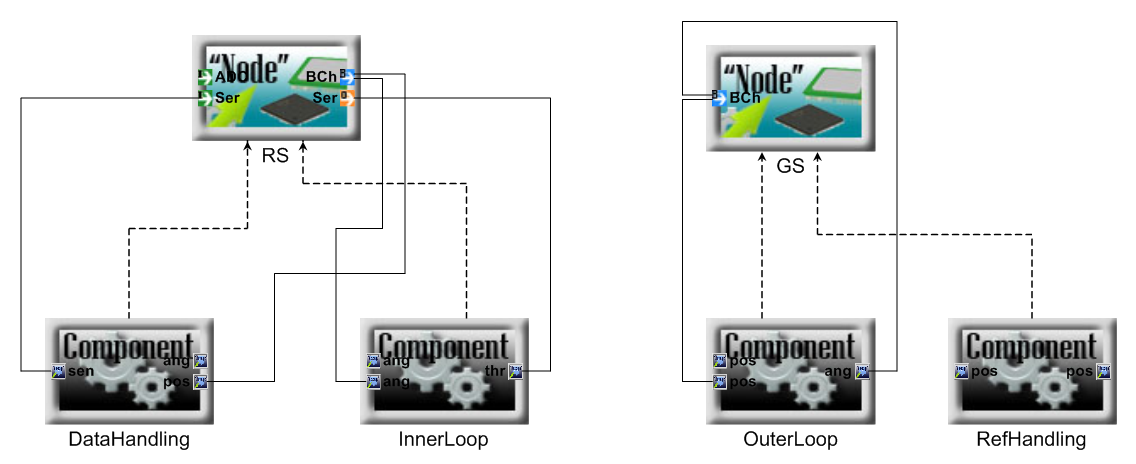
\includegraphics[width=\columnwidth]{figures/quadrotor_hw_mapping}
    \caption{Deployment: The platform mapping model specifies the hardware
components that will support the transfer of data to and from each processing
node, the software components that will send and receive the data, and the
message instances in which the data will be carried.}
    \label{fig:qr_hw_mapping}
\end{figure}

Figs. \ref{fig:qr_log_arch} and \ref{fig:qr_hw_mapping} show different parts of
the GME design model for the quad integrator controller.  The model-integrated
computing approach uses integrated sublanguages to represent models in the
various aspects of the design\cite{mic:overview}. Fig. \ref{fig:qr_log_arch} portrays 
logical data dependencies between software component instances, independent of their 
distribution over different processors. The arrows between the components represent
the transfer of message data. Fig. \ref{fig:qr_hw_mapping} shows the deployment 
model -- the mapping of software components to processing nodes (dashed lines from 
the components to the processors), and data messages to communication ports (solid lines 
between component message interface ports and processor peripheral ports).  RS
(Robostix) is an 8-bit ATMega128 CPU which runs the DataHandling and InnerLoop software
components. GS (Gumstix) is an Intel PXA ARM-based CPU which runs the RefHandling and
OuterLoop components. An execution model (not shown) allows the designer to attach timing 
parameter blocks to components and messages, such as execution period and worst-case execution 
time.  The quad integrator controller runs all of the blocks at a frequency of 50Hz.  
The execution model also indicates which components and messages will be scheduled 
independently, and which will be grouped into a task.  Our example model assigns 
each component to its own task.  All tasks are executed with a static schedule on a 
time-triggered bus.  The static message schedule can introduce additional time delays into
the controller, so delay effects are a concern.

The sector blocks are attached around each controller, so the input and output are from 
the point of view of the control element.  The output of the controller (input to the
rest of the system) is connected to the sector analyzer input port.  The signal controlled by
the controller (before the error term is formed) is part of the input to the controller,
but from our point of view it is the output of the system, so it connects to the sector
analyzer output port.  Fig. \ref{fig:sectorconn} displays the connection of the sector search
around the position control gain for our example. $K_x$ is the proportional gain for the
outer loop PD controller, and $K_v$ is the derivative gain.  Currently the sector blocks are
inserted by hand, as we have not yet completed the modeling extensions for online validation
and input scenarios.

\begin{figure}[htb]
\centering
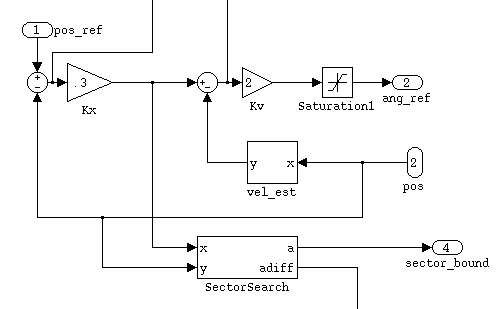
\includegraphics[width=\columnwidth]{figures/sectorconn}
    \caption{Illustration of the sector analysis block connected around the position
controller in the quad integrator test model.  The lines leading off of the figure
correspond to other data taps that are not relevant to illustrate the concept.}
    \label{fig:sectorconn}
\end{figure}
